\chapter{Compute and Virtualization}

\section{Compute Architecture: CPU, GPU and NPU}
Data processing (Compute) is the third pillar of the datacenter. Modern hardware evolution is driven by the end of linear single-core scalability (Moore's Law) and the need for efficiency and specialization for Artificial Intelligence workloads.

\subsection{Energy Sustainability}
Datacenters consume huge amounts of electricity and water. The benchmark metrics are:
\begin{itemize}
    \item \textbf{PUE (Power Usage Effectiveness):} Ratio between the total energy consumed by the datacenter and that actually used by the servers. The ideal value is 1.0.
    \item \textbf{WUE (Water Usage Effectiveness):} Water consumption per kWh, critical in datacenters using evaporative cooling (Cooling towers).
\end{itemize}

\subsection{CPU Architecture: Pipeline and Multi-Core}
Historically, to increase performance, clock frequency was increased and the \textbf{Instruction Pipeline} was optimized (classically divided into phases: \textit{Instruction Fetch, Decode, Execute, Memory Access, Write-back}). By increasing pipeline depth (up to 20+ stages), more overlapping instructions could be executed over time, but \textit{Branch Misprediction} errors caused stalls and complete queue flushing ("bubbles" in the pipeline), nullifying efficiency. 

Having reached the physical limit of dissipatable heat (Power Wall), the shift was made to Multi-Core parallelism. To overcome RAM sharing bottlenecks, modern CPUs adopt \textbf{NUMA (Non-Uniform Memory Access)} architectures, where each processor has its own local memory bank with fast direct access; access to the RAM of other processors occurs via external interconnects with higher latency.

\textbf{Hyperthreading and SMT (Simultaneous Multithreading)}\\
To minimize idle times when a core waits for data from memory, designers introduced \textbf{Hyperthreading} (or SMT). The trick is to duplicate only "lightweight" resources (like registers and the program counter), while sharing the expensive physical calculation units (ALU). The operating system sees \textbf{two logical cores} for each physical core: when a thread stalls for a \textit{cache miss}, the core instantly switches context and executes the other thread's instructions.
Although excellent for web servers and high I/O databases, HT is \textbf{harmful in HPC} (High Performance Computing): if two threads must perform intensive simultaneous mathematical calculations, they will fiercely fight for the single shared ALU, reducing overall performance. Therefore, in supercomputers, HT is disabled.

\begin{tipbox}[Overbooking and Memory Ballooning]
Virtualization relies on \textbf{Overbooking} (logical over-allocation of underlying physical resources). In addition to the obvious over-commit of vCPUs, heavy RAM overbooking is performed. A key mechanism is \textbf{Memory Ballooning}: the hypervisor injects a balloon driver into the guest OS kernel. If the physical server is running out of real RAM, the hypervisor "inflates" the balloon. The guest OS believes it urgently needs internal memory, swaps its least used processes to its virtual disk, and returns the real RAM to the balloon (and therefore to the hypervisor). The hypervisor also masks huge amounts of RAM via \textit{Memory Page Sharing} (e.g., KSM deduplicates identical operating system pages across dozens of identical Windows VMs).
\end{tipbox}

\begin{warningbox}[Side-Channel Vulnerabilities]
Physically sharing the L1 cache and execution buffers between two threads opens the door to speculative attacks like \textbf{Spectre} or \textit{MDS}. A malicious thread can infer the "sibling" thread's secret data by measuring cache latency. For maximum security, some cloud providers disable SMT entirely.
\end{warningbox}

\begin{figure}[H]
    \centering
    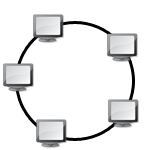
\includegraphics[width=0.6\textwidth]{images/ring_topology.png}
    \caption{Logical diagram of a Ring topology, historically used for internal CPU core interconnection.}
\end{figure}
\textbf{Internal Interconnect: Crossbar vs Bus}\\
At the internal interconnection level (die), early multi-core CPUs used a \textit{Shared Bus}, which immediately became a bottleneck: only one core at a time could talk. Today, the \textbf{Crossbar} (or a \textit{Mesh Network}) is used: an interconnection matrix that allows multiple cores to communicate simultaneously with different memory banks or I/O without interfering, ensuring full \textit{bisection bandwidth}.

This reticular approach pairs perfectly with the \textbf{Tile (or Chiplet)} architecture: modern processors are no longer a single silicon monolith prone to defects, but a mosaic of small hyperspecialized chips (Compute Tile, I/O Tile) printed with different nodes and glued onto the same package, vastly improving production yields and lowering costs. Concrete examples of this approach are the \textbf{AMD Infinity Fabric} interconnect fabric used to join chiplets in EPYC processors, and advanced 3D packaging technologies like \textbf{Intel EMIB and Foveros} (used in Meteor Lake and Sapphire Rapids architectures) that stack silicon dies vertically.

\subsection{GPU and NPU: The Paradigm Shift}
\begin{itemize}
    \item \textbf{CPU:} Optimized for \textit{minimum latency}. Few very complex cores with \textit{Out-of-Order} execution and large caches.
    \item \textbf{GPU:} Optimized for \textit{maximum throughput}. Thousands of simple cores executing the same calculation in parallel (SIMT), ideal for AI training.
    \item \textbf{NPU (Neural Processing Unit):} Dedicated circuits specialized exclusively in tensor calculation and AI inference at low numerical precision and ultra-low power consumption.
\end{itemize}

\section{Physical Server Architectures and BMC}
The physical enclosure (form factor) of servers has diversified over the years to meet different needs for density, computing power, and thermal dissipation.

\subsection{Rack Servers (1U / 2U)}
\begin{figure}[H]
    \centering
    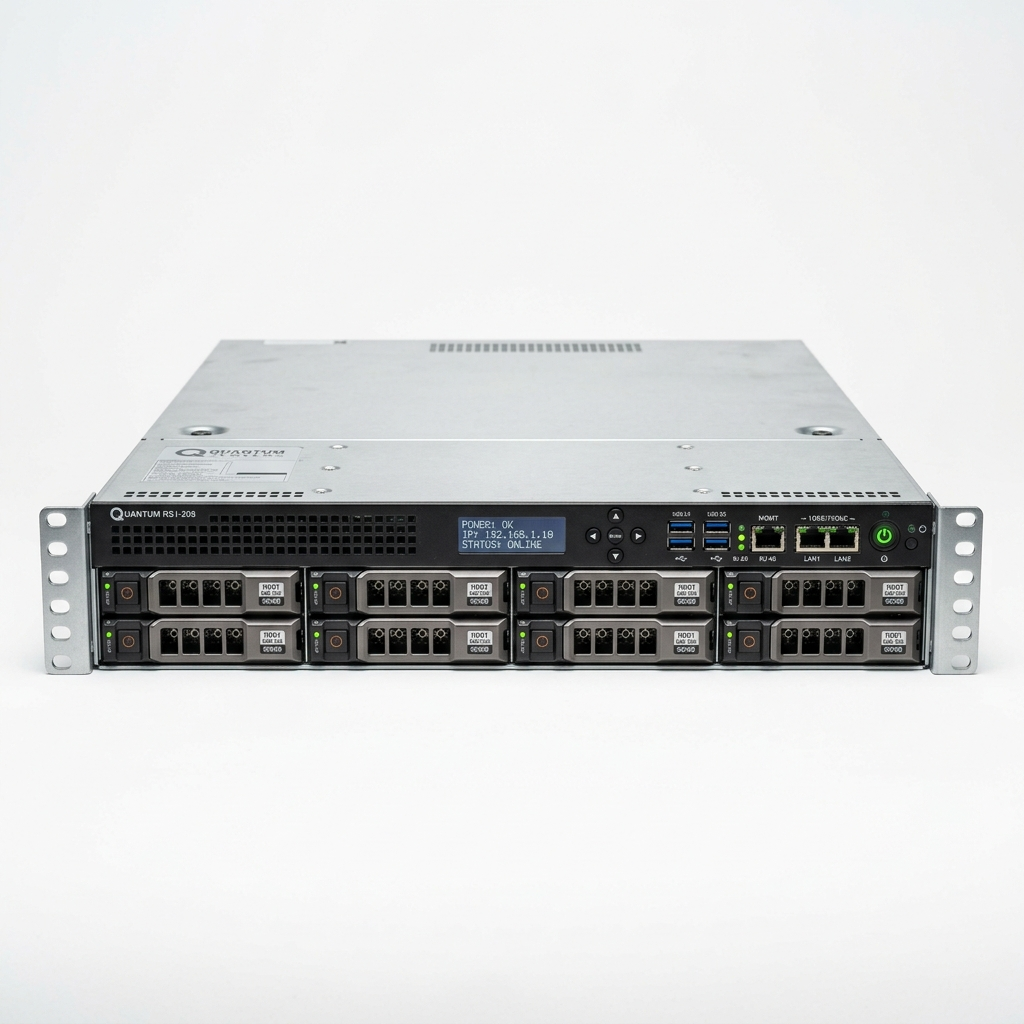
\includegraphics[width=0.7\textwidth]{images/rack_server_1u.png}
    \caption{Standard 1U Rack Server with front hot-swap disk bays.}
\end{figure}
It is the most common "general-purpose" format in traditional data centers. A rack server is a complete and independent computer (equipped with its own power supplies, fans, CPU, RAM and disks) enclosed in a standardized 19-inch wide metal chassis. The height is measured in rack units (U, about 4.4 cm). They are ideal for heterogeneous workloads, but in large quantities they require an enormous amount of individual cabling work for each machine (separate power and network cables for each individual server).

\subsection{Blade Servers}
\begin{figure}[H]
    \centering
    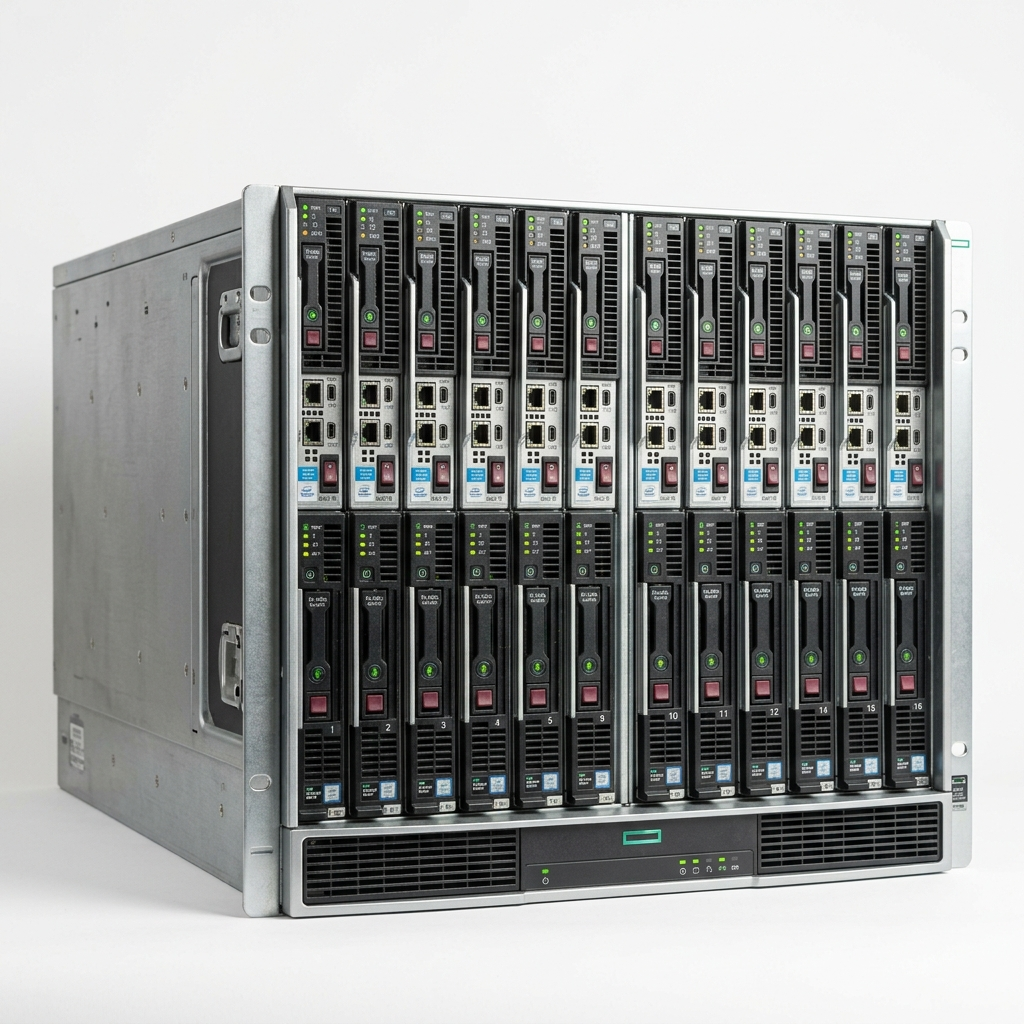
\includegraphics[width=0.7\textwidth]{images/blade_server.png}
    \caption{Blade System Chassis: dozens of server blades inserted into a single module.}
\end{figure}
Designed to achieve the ultra-high density needed in virtualization clusters. A Blade system is divided into two components: the \textbf{Chassis} (the outer enclosure providing shared power, mega-fans and integrated network switches) and the \textbf{Blades} (the actual servers). The Blade is very thin because it only contains CPU, RAM and a few disks; it has no fans or power supplies of its own. By inserting it into the chassis, it automatically connects to the rear \textit{midplane}, almost completely eliminating cabling clutter in the rack.

\subsection{HGX Servers (AI GPU Server)}
\begin{figure}[H]
    \centering
    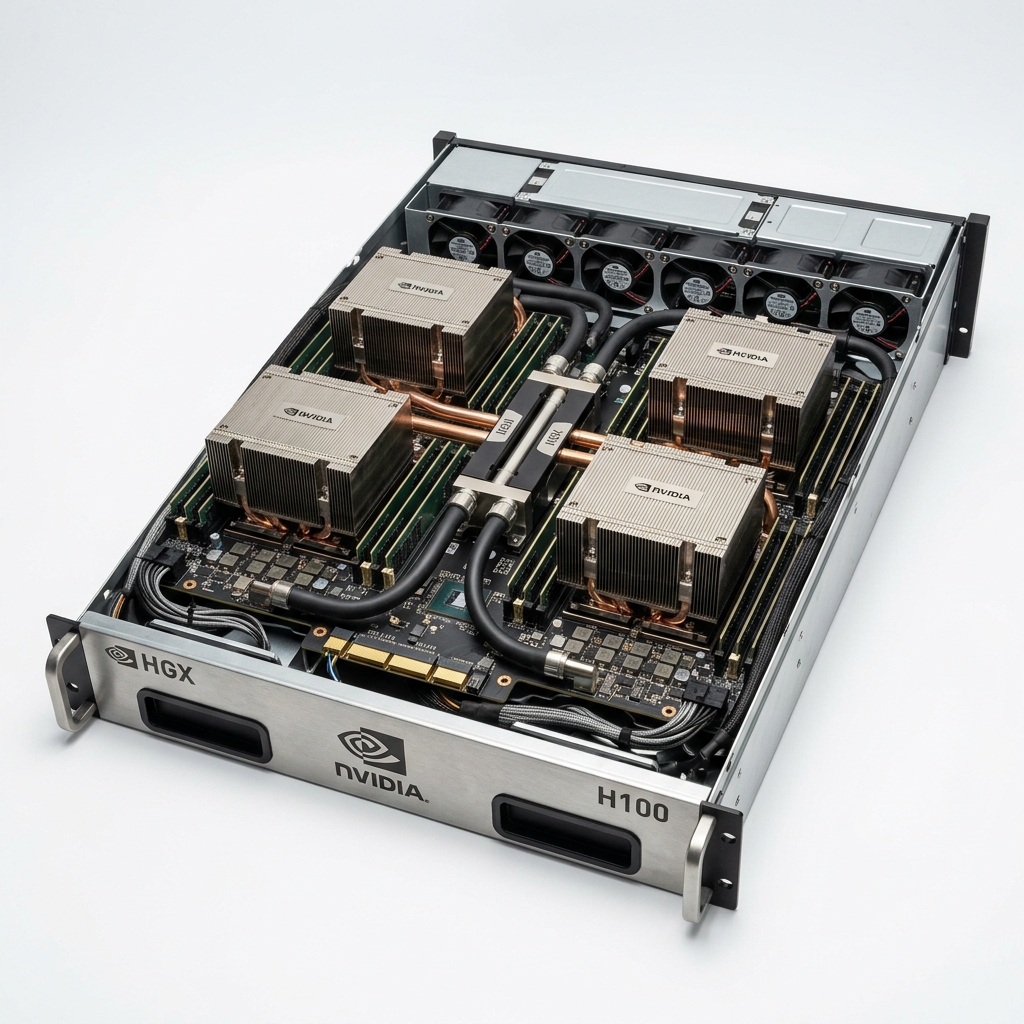
\includegraphics[width=0.7\textwidth]{images/hgx_gpu_server.png}
    \caption{HGX Server (open): high-performance GPUs covered by massive metal heatsinks to handle extreme heat.}
\end{figure}
With the explosion of generative artificial intelligence, regular rack servers are no longer sufficient. An HGX server is a massive machine (often 4U or 8U, weighing over 100 kg) designed exclusively around GPUs (e.g., NVIDIA H100). GPUs are no longer inserted as removable PCIe cards, but are soldered directly onto a proprietary \textit{baseboard} and interconnected via dedicated buses (like NVLink) that bypass the PCIe bottleneck. They generate frightening heat, often making the switch to liquid cooling (\textit{Direct-to-Chip Liquid Cooling}) mandatory.

\subsection{Hyperscaler Standardization: Open Compute Project (OCP)}
Originally created by Meta (Facebook) in 2011, the \textbf{OCP (Open Compute Project)} is a non-profit consortium that publishes open source hardware specifications for datacenter servers and racks. The idea stems from an economic need: traditional branded servers contain many aesthetic or management features (plastic bezels, displays, redundant power supplies per single server) that are useless on a hyperscaler scale.
OCP specifications define essential machines (often produced directly by Taiwanese ODM manufacturers like Quanta or Foxconn), allowing for enormous savings. A key OCP innovation is the rack design: power is not converted in every single server, but centralized upstream in the rack and distributed to the servers via 12V or 48V busbars, increasing energy efficiency and density.

\begin{tipbox}[BMC (Baseboard Management Controller) and the Redfish Standard]
All enterprise-grade servers are equipped with a \textbf{BMC} (e.g. HPE's iLO or Dell's iDRAC). It is an independent micro-computer inserted into the motherboard, equipped with a dedicated network port (\textit{out-of-band management}). Being separately powered, it allows physical control of the server (power on, BIOS configuration, virtual KVM console) even if the main operating system is frozen or if the server is physically powered off.

\textbf{Redfish: The Modern Datacenter API}\\
Historically, BMCs were managed via the IPMI protocol, which over time proved to be insecure and difficult to integrate. For this reason, the DMTF consortium introduced \textbf{Redfish}, the modern standard for infrastructure management.
\begin{itemize}
    \item \textbf{How it works:} Redfish exposes all hardware parameters via a standard \textbf{RESTful API}. It uses modern web protocols (HTTPS for security) and returns data in \textbf{JSON} (OData) format, easily readable by both humans and scripts.
    \item \textbf{What it does:} It allows automating the most tedious operations on a large scale. Through simple Python scripts or tools like Ansible, web requests (GET, POST, PATCH) can be sent to monitor temperatures, update firmware, change the boot order or restart an entire rack of servers, regardless of the underlying hardware brand.
\end{itemize}
\end{tipbox}

\section{Virtualization and Live Migration}
Virtualization decouples software from physical hardware, allowing multiple Operating Systems (Guests) to run simultaneously on the same physical server (Host). The heart of this process is the \textbf{Hypervisor} (or Virtual Machine Monitor).

\subsection{Hypervisor Evolution: From CPU Rings to Hardware Virtualization}
The original x86 architecture was not designed to be virtualized. It provided four logical privilege levels called \textbf{Rings}, from Ring 0 (maximum privilege, intended for the OS kernel) to Ring 3 (user space). 
In a virtualized environment, the Hypervisor must have absolute control, therefore it must reside in Ring 0. This forced Guest operating systems to scale into Ring 1 (unprivileged mode, defined as \textit{Ring De-privileging}). Since Guest OSes did not know they were virtualized, they attempted to execute privileged instructions (e.g., hardware manipulation) which, failing, were trapped by the Hypervisor. The latter had to translate and emulate them in real time (\textbf{Binary Translation} technique), causing huge and unsustainable performance overhead.

The problem was solved in 2005 by CPU manufacturers with the introduction of dedicated hardware extensions (\textbf{Intel VT-x} and \textbf{AMD-V}). These instructions created a new privilege level below zero (often colloquially called \textbf{Ring -1}). Today the Hypervisor resides in Ring -1, allowing Guest operating system kernels to operate in their native Ring 0, executing instructions directly and at hardware speed, eliminating the need for slow binary translation.

\subsection{Hardware Abstraction: vCPU, Pause and Resume}
The virtual machine does not see the real physical CPU, but a \textbf{vCPU} (Virtual CPU) configured by the hypervisor. This is a crucial detail for portability: the hypervisor can hide overly recent instruction sets (e.g. AVX-512) by masking the true capabilities of the physical processor, so that the VM can be freely migrated even to an older server that does not possess those instructions. 

Furthermore, since the entire Guest environment is just software running on a controlled \textit{fetch-execute} cycle, the hypervisor enjoys the power of \textbf{Pause and Resume}. It can instantly freeze the operating system by saving \textit{the complete state of the VM} (CPU registers, memory state and virtual disk). The virtualized OS will notice nothing; for it, time will have simply stopped. 
Through \textbf{Integration Services}, the hypervisor then forces clock synchronization upon resumption (vital for protocols like Kerberos which fail if the time is desynchronized), sends \textit{heartbeat} signals to understand if the Guest kernel has crashed, and orchestrates graceful shutdowns.

\begin{tipbox}[Windows Dual Boot and Secure World with WSL2]
Today virtualization is pervasive even on client devices. Upon startup, a modern Windows PC (VBS enabled) does not perform a normal bare-metal boot, but launches a hypervisor (Hyper-V) that instantiates two environments. The first is a hidden micro-OS (\textbf{Secure World}) that isolates cryptographic hardware (e.g. BitLocker keys). Immediately after, the main desktop Windows environment is launched, which therefore runs \textit{virtualized}. Even if a hacker obtains maximum privileges (Ring 0) on the Windows kernel, they can never steal the Secure World's cryptographic keys.
The same transparent client hypervisor makes \textbf{WSL2} (Windows Subsystem for Linux) possible, which runs a true, complete Linux kernel in an ultra-light micro-VM alongside Windows.
\end{tipbox}

\subsection{The Virtual Switch (vSwitch)}
To connect VMs to the outside world, the Hypervisor implements a \textbf{Virtual Switch} in RAM. Virtual machines possess logical network interface cards (\textbf{vNICs}), which connect to the vSwitch ports. In turn, the vSwitch routes traffic to the physical network via the server's real network interface cards (\textbf{pNICs}). The vSwitch manages complex logic in software such as VLAN tagging, traffic shaping, and physical interface teaming in a way that is completely transparent to the guest virtual machines.

\subsection{Live Migration}
The most disruptive feature of virtualization is \textbf{Live Migration} (e.g. VMware vMotion), which allows moving a running VM from one physical host to another without service interruption.
It rigorously develops in three sequential phases:
\begin{enumerate}
    \item \textbf{Pre-copy (Dirty tracking):} Initial massive memory transfer while the VM runs on the old host. The system actively tracks via a bitmap (\textit{dirty page tracking}) which memory pages are modified during the slow network copy operation. This cycle is repeated to transfer subsequent deltas.
    \item \textbf{Stop and copy:} When very few dirty pages remain, the VM is "frozen" (imperceptible pause of a few ms). The residual state of CPU registers, I/O buffers, and residual RAM is copied. Execution is transferred to the destination hypervisor.
    \item \textbf{Network Management (Gratuitous ARP):} Since the VM's MAC address has physically moved to another port of the datacenter core switch, the destination vSwitch sends a broadcast \textbf{Gratuitous ARP}. This instantly updates the CAM tables of all physical switches, ensuring that in-transit packets are not lost.
\end{enumerate}

\section{Containerization}
Unlike virtualization, \textbf{Containers} do not emulate entire hardware or an entire kernel, but \textbf{share the host's Linux kernel}. This reduces overhead to zero, but radically changes security and networking modes.

\subsection{Isolation Mechanisms and Vulnerabilities}
Isolation, vital to prevent containers from collapsing into each other, is delegated to the operating system kernel via two primitives:
\begin{itemize}
    \item \textbf{Namespaces:} Isolate logical visibility. A namespace makes the container believe it is the only system, giving it an independent PID tree and exclusive mount points.
    \item \textbf{Cgroups (Control Groups):} Limit hardware usage (impose strict CPU ceilings or strict \textit{OOM killers} for RAM).
\end{itemize}

Sharing the kernel means, however, that a flaw in it affects everyone simultaneously. The course cites the anomalous case of the \textbf{CVE-2026-31431 ("Copy Fail")} vulnerability in the \texttt{authencesn} module: by abusing the \textit{page cache} shared between containers, a trivial Python script allows not only privilege escalation, but a catastrophic \textit{container escape}, jeopardizing entire orchestration nodes.

\subsection{Docker Architectural Details}
\begin{itemize}
    \item \textbf{Overlay File System:} Containers use layered file systems (e.g. \textit{overlay fs}). The container image is immutable (read-only). By starting it, a lightweight ephemeral \textit{Read-Write} layer is created on top. Modifying a base file triggers a slow \textit{Copy-on-Write} to the upper layer.
    \item \textbf{Multi-stage Build:} In modern software development, a giant container is used to compile source code. Then, a second stage copies only the final compiled binary into an empty image (e.g. 5MB Alpine Linux), drastically reducing the footprint and attack surface.
    \item \textbf{Hardware Drivers distributed via Container:} Even complex drivers are being "containerized". NVIDIA, to facilitate AI deployments on bare-metal nodes, distributes the NVIDIA Container Toolkit, encapsulating GPU drivers and CUDA libraries in an isolated container instead of installing them on the host.
\end{itemize}

\subsection{Network: VM vs Container}
In virtual machines, the hypervisor creates an isolated \textbf{vNIC} (a real fake card visible to the VM) and connects it to the vSwitch. 
In containers, this abstraction is missing. Instantiated containers (if they don't use complex bridges like in K8s) \textbf{directly contend for access to the pNIC} (physical card of the host) via internal routing. For this reason, containers need \textbf{Port Mapping}: the internal port of the daemon (e.g., NGINX's 80) must be mapped and translated via NAT to another exposed port on the host server.

\begin{figure}[H]
    \centering
    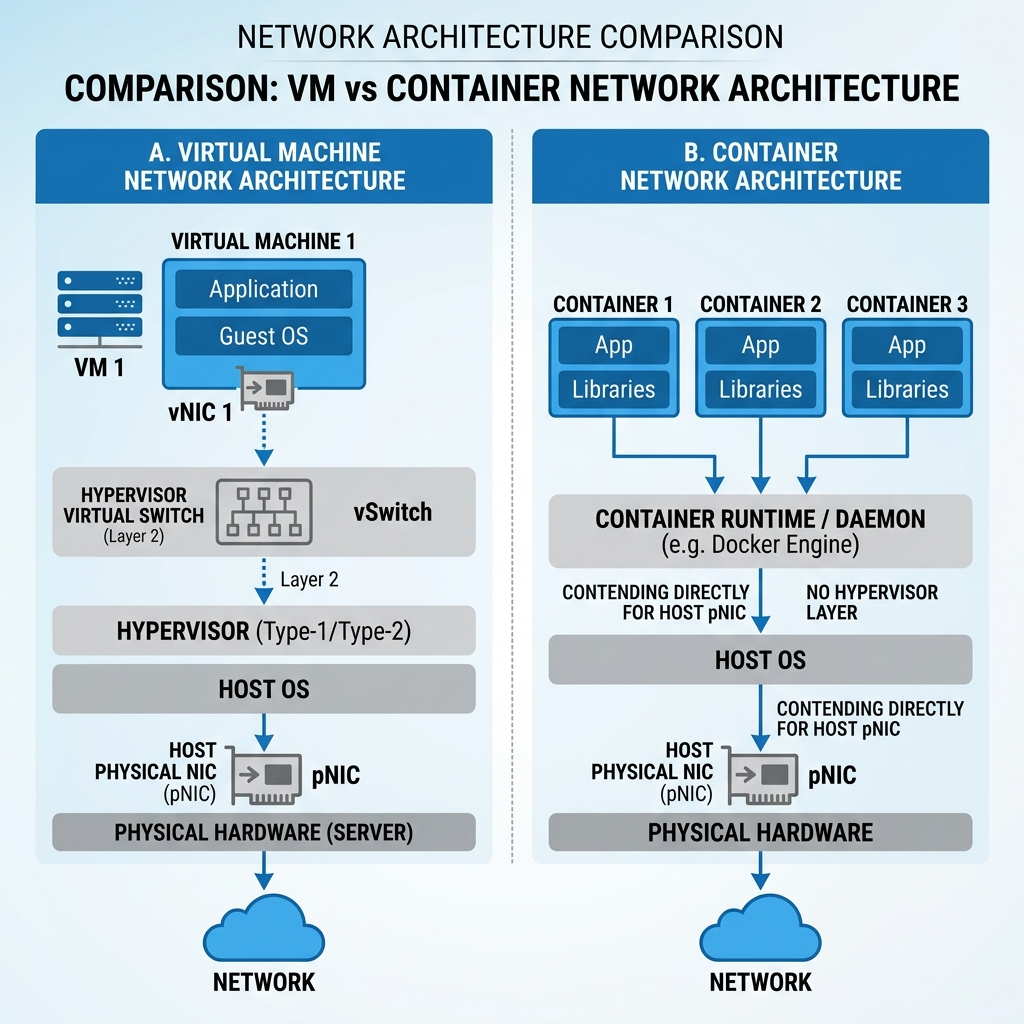
\includegraphics[width=0.8\textwidth]{images/container_vm_network.png}
    \caption{Network architecture: vNIC abstraction (VM) vs contention and NAT (Container).}
\end{figure}

The integration of Containers and Virtualization is, however, the standard: the cloud often runs Kubernetes clusters composed of \textit{Worker nodes} that are themselves virtual machines, thus combining the lightness and deployment ease of containers with the robust hardware isolation (preventing container escape) of VMs.
